% Golden Rule One, Exercise 
%
% The purpose of the exercise is to demonstrate that even small,
% apparently simple, datasets can have surprising properties. In 
% particular, we demonstrate that it can be unwise to trust only
% summary statistics, without inspecting the underlying distribution
% of data

\subsection{Golden Rule 1 Exercise}
\begin{frame}
  \framesubtitle{Subgroups}
  \begin{itemize}
    \item You are in group A, B, C or D - this decides your dataset: \\
             \texttt{expnA.tab}, \texttt{expnB.tab}, \texttt{expnC.tab}, \texttt{expnD.tab}
    \item You will use \texttt{R} at the command-line to analyse your data
  \end{itemize}
\end{frame}
  
\begin{frame}
  \frametitle{Exercise 1}
  \framesubtitle{The biological question}
  \begin{itemize}
    \item Your dataset \texttt{expn?.tab} describes (log) expression data for two genes: \texttt{gene1} and \texttt{gene2}
    \item Expression measured at eleven time points (including control)
    \item Q: Are \texttt{gene1} and \texttt{gene2} genes coregulated?
    \item How do we answer this question?
  \end{itemize}
\end{frame}  

\begin{frame}
  \frametitle{Exercise 1}
  \framesubtitle{Reformulating the question}
  \begin{itemize}
    \item<1-> Q: Are \texttt{gene1} and \texttt{gene2} genes coregulated?
    \item<1-> A: We cannot determine this from expression data alone
    \item<2-> Reformulate the question:
    \item<2-> NewQ: Is there evidence that \texttt{gene1} and \texttt{gene2} expression profiles are correlated? \\
                   (is expression \texttt{gene1} $\propto$ \texttt{gene2})
    \item<2-> How do we answer this new question?
  \end{itemize}
\end{frame}

% [fragile] frames must end with \end{frame} directly following a newline, or they break!
\begin{frame}[fragile]
  \frametitle{Exercise 1}
  \framesubtitle{Starting the analysis}
  \begin{itemize}
    \item Change directory to where Exercise 1 data is located, and start R.
  \end{itemize}
\begin{lstlisting}[language=bash]
$ cd ../../data/ex1_expression/
$ R
\end{lstlisting}
\end{frame}

% [fragile] frames must end with \end{frame} directly following a newline, or they break!
\begin{frame}[fragile]
  \frametitle{Exercise 1}
  \framesubtitle{Load and inspect data in R}
\begin{lstlisting}[language=R]
> data = read.table("expnA.tab", sep="\t", header=TRUE)
> head(data)
  gene1 gene2
1    10  8.04
2     8  6.95
3    13  7.58
4     9  8.81
5    11  8.33
6    14  9.96
\end{lstlisting}
  %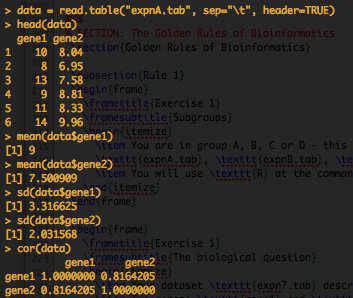
\includegraphics[width=.5\textwidth]{images/ex1_screenshot_b}
\end{frame}

% [fragile] frames must end with \end{frame} directly following a newline, or they break!
\begin{frame}[fragile]
  \frametitle{Exercise 1}
  \framesubtitle{Load and inspect data in R}
\begin{lstlisting}[language=R]
> mean(data$gene1)
[1] 9
> mean(data$gene2)
[1] 7.500909
> sd(data$gene1)
[1] 3.316625
> sd(data$gene2)
[1] 2.031568
> cor(data)
          gene1     gene2
gene1 1.0000000 0.8164205
gene2 0.8164205 1.0000000
\end{lstlisting}
  %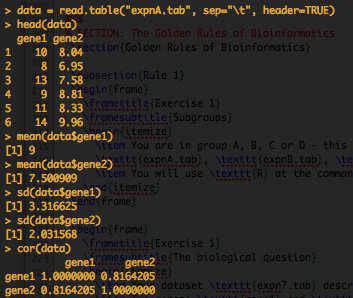
\includegraphics[width=.5\textwidth]{images/ex1_screenshot_b}
\end{frame}

\begin{frame}
  \frametitle{Exercise 1}
  \framesubtitle{Results}
  \begin{center}
  \begin{tabular}{r|l|l|l|l}
          measure & expnA & expnB & expnC & expnD \\
	  \hline
	  mean(gene1) & 9     &  &  & \\
	  mean(gene2) & 7.5   &  &  & \\
  	  sd(gene1)   & 3.3   &  &  & \\
  	  sd(gene2)   & 2.0   &  &  & \\  
	  cor(data)   & 0.816 &  &  & \\  
  \end{tabular}
  \end{center}
\end{frame}

\begin{frame}
  \frametitle{Exercise 1}
  \framesubtitle{Results}
  \begin{center}
  \begin{tabular}{r|l|l|l|l}
	  measure & expnA & expnB & expnC & expnD \\
	  \hline
	  mean(gene1) & 9     & 9     & 9     & 9 \\
	  mean(gene2) & 7.5   & 7.5   & 7.5   & 7.5 \\
  	  sd(gene1)   & 3.3   & 3.3   & 3.3   & 3.3 \\
  	  sd(gene2)   & 2.0   & 2.0   & 2.0   & 2.0 \\  
	  cor(data)   & 0.816 & 0.816 & 0.816 & 0.816 \\  
  \end{tabular}
  \end{center}
  \begin{itemize}
     \item<2-> $r=0.816 (P<0.005)$ in every experiment
     \item<2-> Can we conclude that \texttt{gene1} and \texttt{gene2} are coexpressed in each experiment?
  \end{itemize}
\end{frame}

% [fragile] frames must end with \end{frame} directly following a newline, or they break!
\begin{frame}[fragile]
  \frametitle{Exercise 1}
  \framesubtitle{Plot the data in R}
\begin{lstlisting}[language=R]
> plot(data)
\end{lstlisting}
  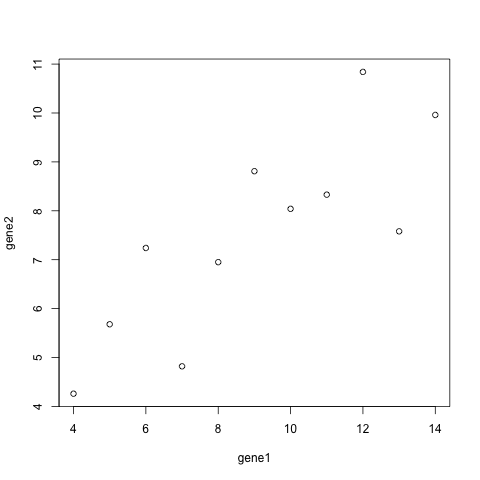
\includegraphics[width=0.4\textwidth]{images/ex1_screenshot_d}        
\end{frame}

\begin{frame}
  \frametitle{Exercise 1}
  \framesubtitle{Always plot the data}
    Which gene pairs are coexpressed?
  \begin{center}
    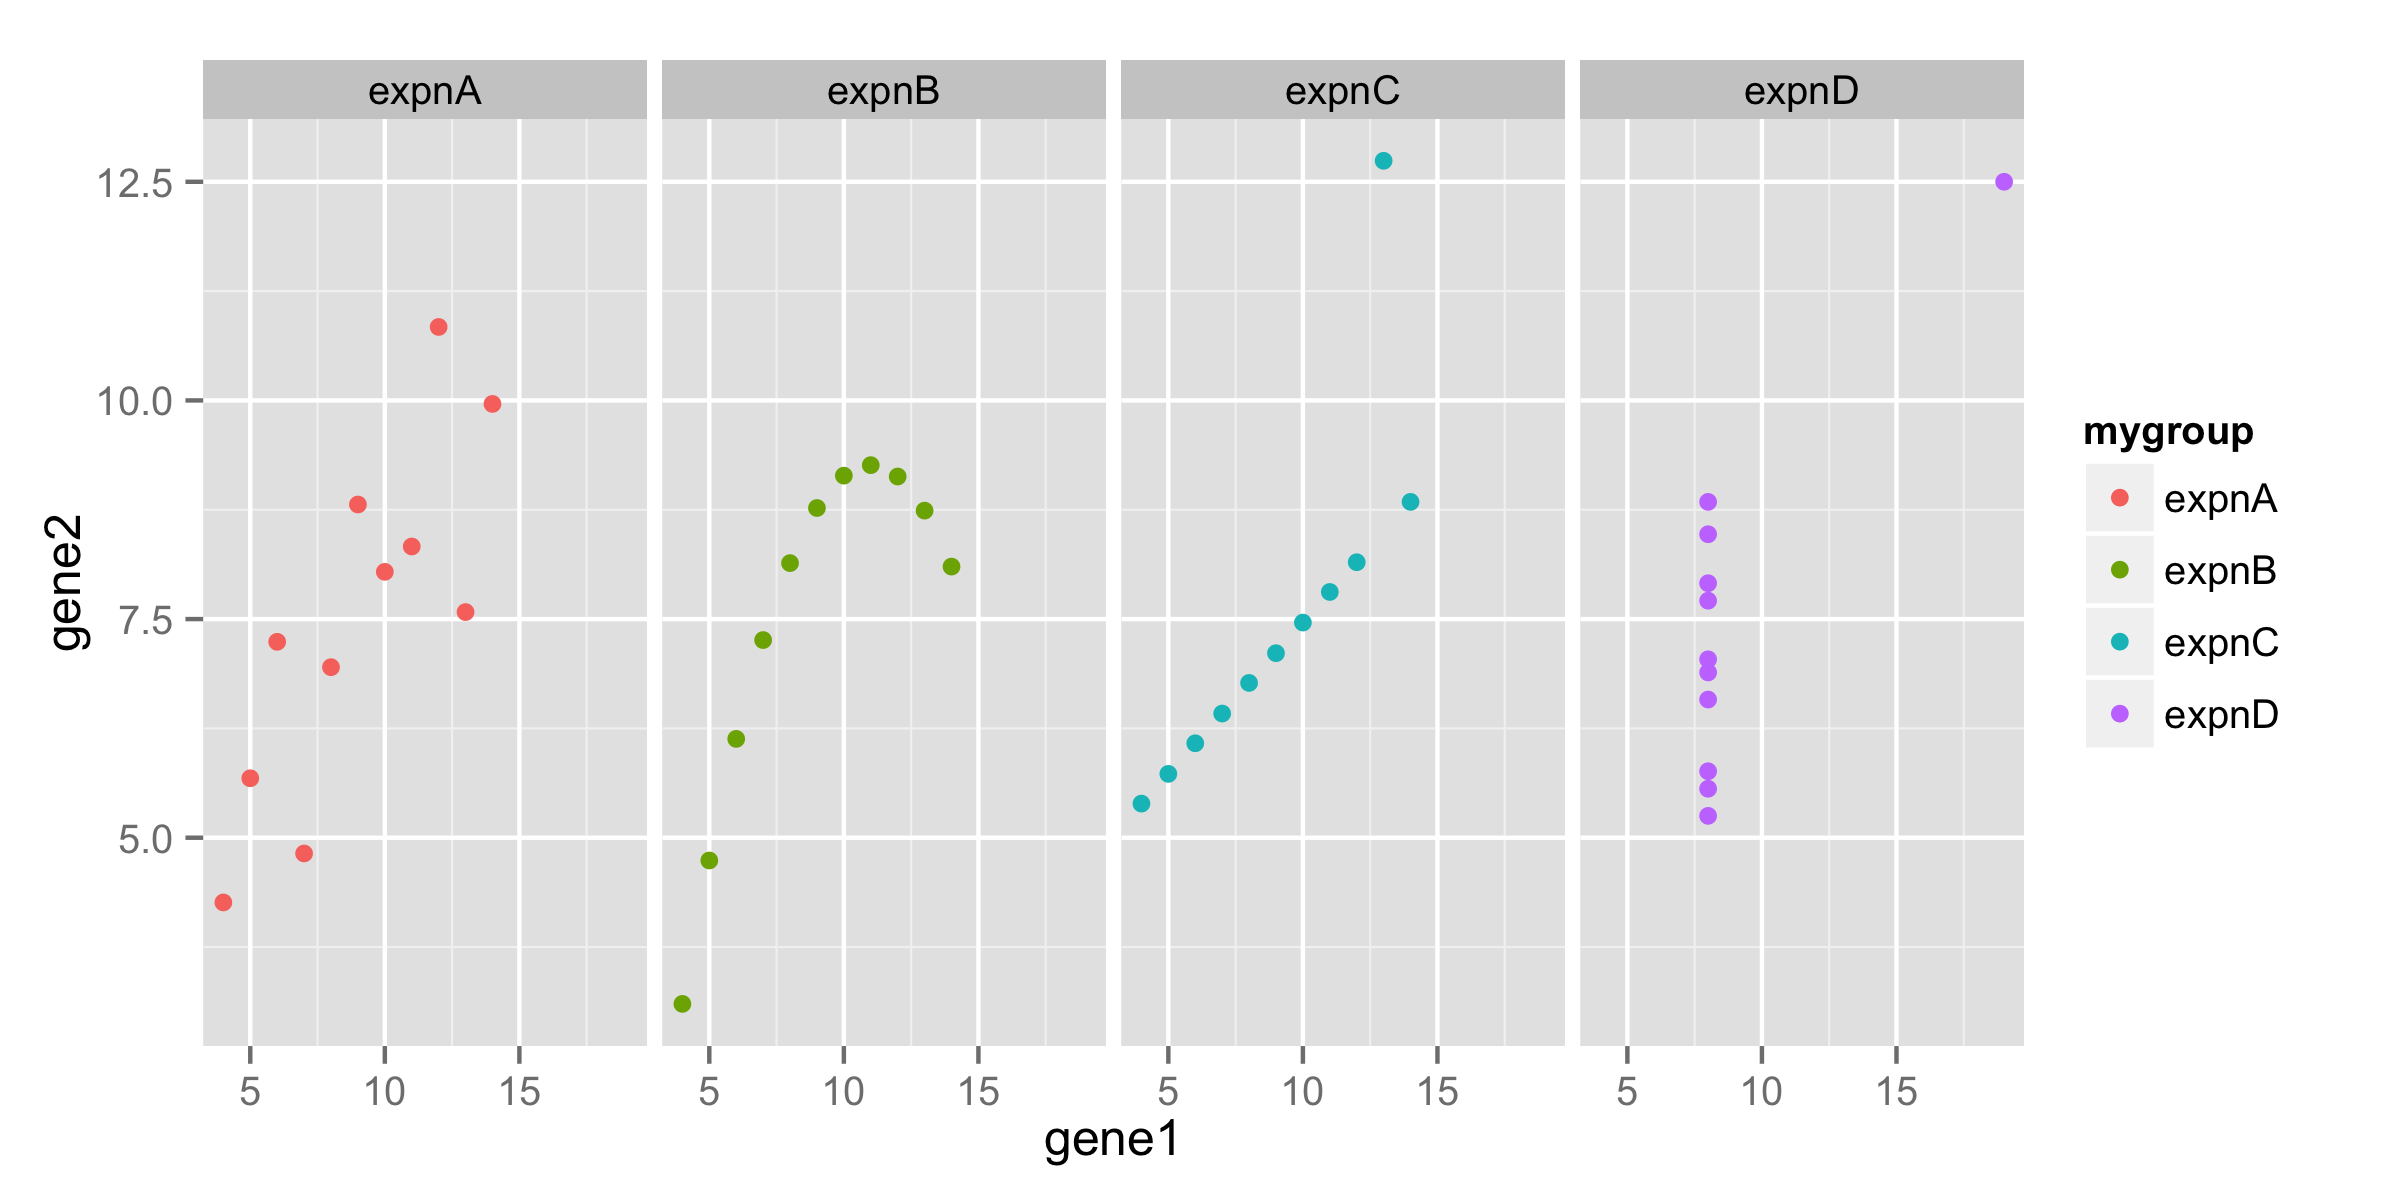
\includegraphics[width=0.9\textwidth]{images/ex1_rplot} \\
  \end{center}
\end{frame}

\begin{frame}
  \frametitle{Exercise 1}
  \framesubtitle{Always plot the data}
    Is a matrix of correlation values potentially misleading?
  \begin{center}
    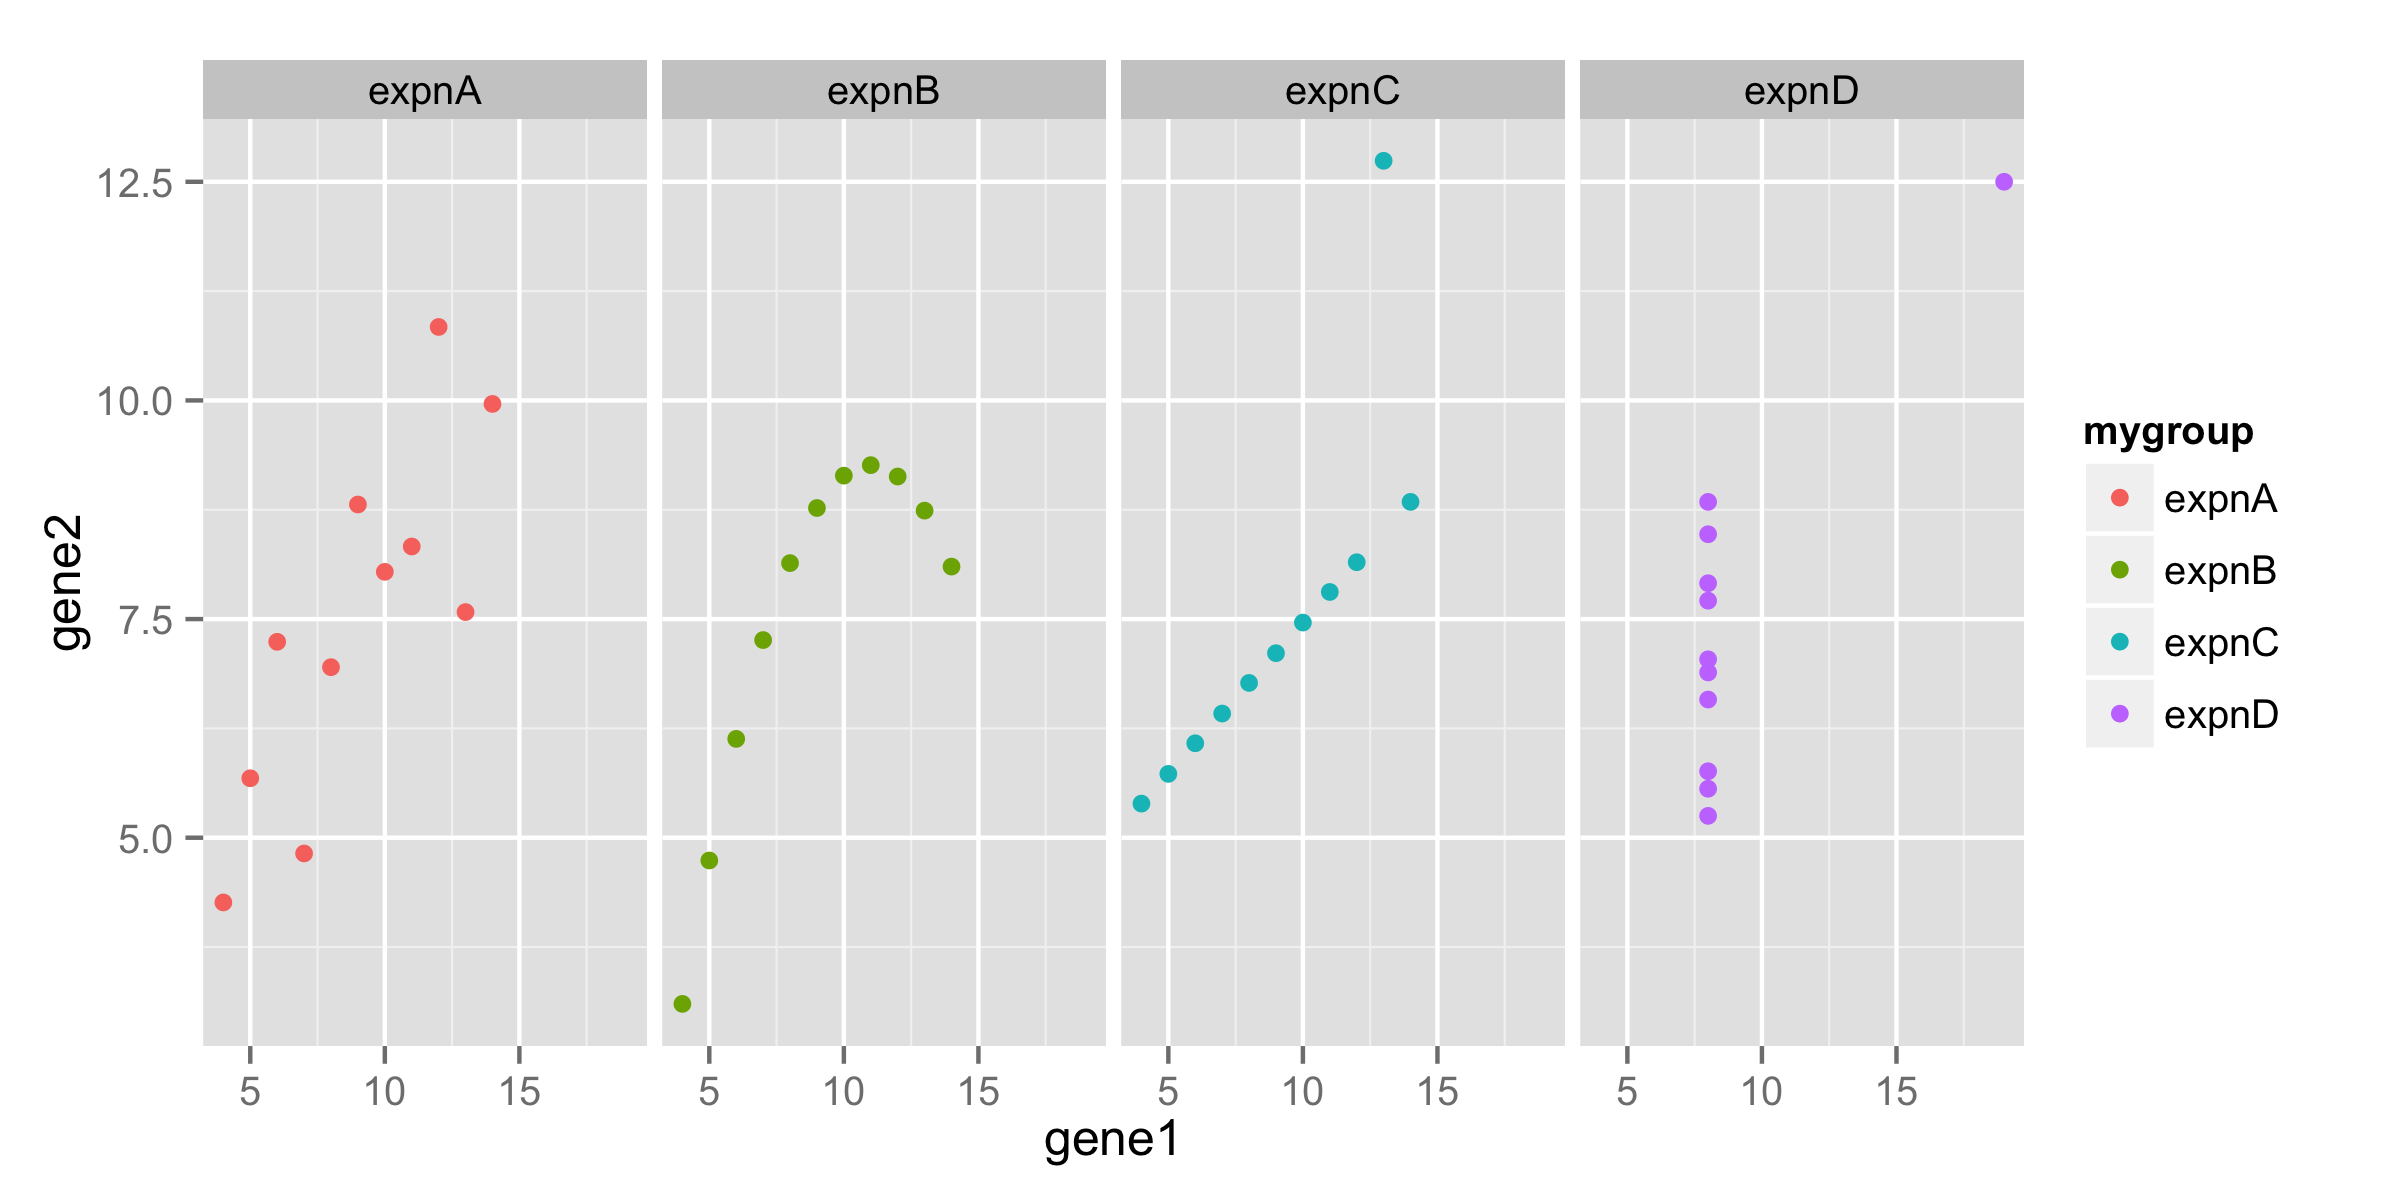
\includegraphics[width=0.9\textwidth]{images/ex1_rplot} \\
  \end{center}
\end{frame}
